\documentclass[11pt]{article}
\usepackage[a4paper,margin=1in]{geometry}
\usepackage{url}
\usepackage{hyperref}
\usepackage{natbib}
\usepackage{amsmath}
\usepackage{graphicx}
\graphicspath{ {./images/} }
\DeclareMathOperator{\logit}{logit}

\title{Dissecting Dota \\[\baselineskip] \large A statistical analysis of DotA 2}

\author{
    Sathkrith, Madhukara S Holla
    \\
    1st year MSCS, Northeastern University
}
\date{December 2023}

\begin{document}
\maketitle
\newpage

\section{Introduction}
Defense of the Ancients (DotA), is a competitive multiplayer video game.
Originally developed as a custom map for Warcraft III, it has evolved into a
standalone title with a massive global player base. Two teams of five players
each engage in strategic battles, navigating a dynamic map and competing against
both minions and enemy players. The ultimate goal is to destroy the enemy
team's Ancient, a crucial structure within their base.
\\

In DotA, each player chooses a hero, with a unique set of skills, contributing
to the diverse team strategies. Players assume distinct roles within the team,
namely "Carry", "Mid", "Offlaner", "Soft support" and "Hard support", commonly
referred to as "Position 1" through "Position 5". The battle unfolds across
three lanes - Top, Mid and Bottom - with each serving as a critical pathway
for advancing towards enemy base. A crucial aspect of gameplay is accruing
gold and experience points, achieved by defeating both minions and enemy heroes.
This process of leveling up heroes and acquired items is central to gaining a
tactical advantage. Additionally, players aim to destroy enemy towers, the
defensive structures in each lane, to establish map control. Successfully
destroying these towers not only weakens the enemy's defenses but also positions
the team more favorably to seize control of the game.
\\

Our study aims to explore different factors that influence a team's chances of
winning a game. The initial focus is on the impact of resource distribution
within a team on their likelihood of winning. This aspect of the investigation
revolves around analyzing the networth ratio as a key parameter, with the
outcome of each game (win or loss) serving as the response variable.
We further explore the influence of other factors, such as the networth of
individual players, kills secured by a player, and towers lost by the team on
the outcome of a match.

\section{Summary of the dataset}
The dataset sources from Stratz\cite{stratzWebsite} comprises of 8,250 matches.
A random walk methodology with restrictions ensured one game per player, all
within the same skill bracket. Post-collection, we preprocessed the data to
remove matches with outliers, NaN values and one-sided games.
The final dataset, reduced to 7500 matches, includes detailed metrics like
player roles, hero choices, resource metrics at various intervals and match
outcomes. Match outcome and hero type are categorical variables, while the
remaining metrics are numerical values. For analysis, the matches were
partitioned into two sets to analyze the winning and losing teams separately,
ultimately focusing on 4,500 matches after considering hero restrictions.
\\

The resource metrics in game are influenced by the duration of the game. Therefore,
the analysis focused on the net worth of the five team positions at 10 and 20
minutes into the game. A crucial aspect was managing the extensive pool of 120
heroes. To ensure a practical and effective analysis, the study limited its focus
to 40 heroes, selected based on their frequency of appearance in the dataset.
This approach prioritized the most commonly chosen heroes, providing a balanced
representation of popular gameplay strategies.

\section{Identifying the key factors}
To identify key factors affecting game outcomes, our approach involved a thorough
analysis of the dataset. We utilized various visualization techniques and statistical
metrics to understand the influence of different variables, such as player roles,
hero choices, and resource metrics, on match results.
(Appendix \ref{sec:datavisualization} for data visualizations)
\\

We eliminated factors with high skewness, direct correlation or high multicollinearity to refine the model.
With results from histograms, boxplots, and a correlation matrix, we selected
the most relevant variables: net worths of the five team positions, towers lost,
and match outcomes at 10 or 20 minutes. There variables are not only statistically
significant but also have practical relevance in the game context.
\\

Additionally, we conducted AIC tests with forward model selection and interaction
tests to validate selected parameters. The AIC tests confirmed the significance
of the selected variables, while the interaction tests revealed no significant
interactions between the variables. The results of these tests are included in
Appendix \ref{sec:aictest} and \ref{sec:interactiontest} respectively.

\section{Methods}
For our analysis, logistic regression was chosen as the statistical model due
to its effectiveness in handling binary response variable - in this case, match
outcomes categorized as wins (1) or losses (0). The model is fit using maximum
likelihood estimation for 10 and 20 minute net worths separately. This model is
ideal for exploring relationships between independent variables, like resource
distribution, and a binary outcome.
\\[\baselineskip]
There are two main questions that we ask in our analysis:
\begin{enumerate}
    \item Is the distribution of in-game resources among players a determining
    factor in the outcome of a match?
    \item Which factors are most crucial in determining a team's likelihood
    of securing a Win?
\end{enumerate}

\subsection{Model 1}
To approach the first question, we use the following logistic regression model:
\[\logit(p) = \beta_0 + \beta_1 \times Ratio_1 + \beta_2 \times Ratio_2 + \beta_3 \times Ratio_3 + \beta_4 \times Ratio_4\]
\[p = \frac{1}{1 + e^{-\logit(p)}}\]
\begin{itemize}
    \item where \(p\) is the probability of a team winning the match
    \item \(Ratio_1\) through \(Ratio_4\) are the ratios of net worths of the
    \(Position_1\) through \(Position_4\) respectively (\(Position_5\) is excluded
    to maintain linear independence - as they sum to 1)
    \item \(\beta_0\) through \(\beta_4\) are the coefficients of the model
\end{itemize}

\subsection{Model 2}
To approach the second question, we used the following logistic regression model
after considering several parameters and running diagnostic tests. (Appendix \ref{sec:diagnostictest})
\[\logit(p) = \beta_0 + \beta_1 \times NW_1 + \beta_2 \times NW_2 + \beta_3 \times NW_3 + \beta_4 \times NW_4 + \beta_5 \times NW_5 + \beta_6 \times Towers\]
\[p = \frac{1}{1 + e^{-\logit(p)}}\]
\begin{itemize}
    \item where \(p\) is the probability of a team winning the match
    \item \(NW_1\) through \(NW_5\) are the absolute net worths of the five team positions
    \item \(Towers\) is the number of towers lost
    \item \(\beta_0\) through \(\beta_6\) are the coefficients of the model
\end{itemize}

\subsection{Model selection}
To find an appropriate model, we ran diagnostic tests on every possible
parameter combination. Out first step was to eliminate models with residual
deviations greater than 0.3 from the horizontal line. Following this residual-based
filterting, we added an additional criterion by removing models with low
Area Under the Curve (AUC) values.
\\

Following that, we prioritized ten models based on their Akaike Information
Criterion (AIC) scores. To reach a final decision, we manually examined these
ten models, choosing the one that exhibited the most favorable residual vs.
probability graph.

\section{Results}
\subsection{Model 1}
The analysis outcomes primarily stem from the likelihood test and Wald tests
conducted on the model parameters. In the likelihood test, the reduced model
consists of only the intercept as a parameter, serving as a baseline for comparison.

\begin{itemize}
    \item \textbf{Null Hypothesis}: The networth ratios of the five team positions
    do not affect the outcome of the match.
    \\ \(H_0: \beta_1 = \beta_2 = \dots = \beta_4 = 0\)
    \item \textbf{Alternate Hypothesis}: The networth ratios of atleast one position
    affects the outcome of the match.
    \\ \(H_1: \beta_i \neq 0\) for at least one \(i\)
\end{itemize}
\begin{table}[h]
    \centering
    \begin{tabular}{|c|c|}
        \hline
        \textbf{Likelihood test: Full model vs Reduced model} & \textbf{Result} \\
        \hline
        Test statistic (chi-squared) & -1128 \\
        p-value & $< 0.001$ \\
        \hline
    \end{tabular}
\end{table}
The p-value is less than 0.001, which shows that not all parameters are zero.
\\[\baselineskip]
We performed a Wald test for each individual parameter to assess its significance.
The findings suggest that the distribution of resources among different roles does
not influence the probability of winning
\begin{table}[h]
    \centering
    \begin{tabular}{|c|c|c|}
        \hline
        \textbf{Parameter} & \textbf{Value} & \textbf{p-Value} \\
        \hline
        Position 1 Net-worth Ratio & -2.38 & 0.66\\
        Position 2 Net-worth Ratio & -1.5 & 0.78\\
        Position 3 Net-worth Ratio & -3.99 & 0.47\\
        Position 4 Net-worth Ratio & -4.48 & 0.42\\
        \hline
    \end{tabular}
\end{table}
where the p-Values correspond to the result of the Wald test on the parameter.

\subsection{Model 2}
Similar to model 1, the results of the analysis are the results of likelihood test
and Wald tests.
\begin{itemize}
    \item \textbf{Null Hypothesis}: The absolute networth of the five team positions
    and the number of towers lost do not affect the outcome of the match.
    \\ \(H_0: \beta_1 = \beta_2 = \dots = \beta_6 = 0\)
    \item \textbf{Alternate Hypothesis}: Atleast one of the parameters affects the
    outcome of the match.
    \\ \(H_1: \beta_i \neq 0\) for at least one \(i\)
\end{itemize}
\begin{table}[h]
    \centering
    \begin{tabular}{|c|c|}
        \hline
        \textbf{Likelihood test: Full model vs Reduced model} & \textbf{Result} \\
        \hline
        Test statistic (chi-squared) & 1782 \\
        p-value & $< 0.001$ \\
        \hline
    \end{tabular}
\end{table}
Likelihood test indicates that not all parameters are zero.
\\[\baselineskip]
Results of Wald test on each parameter:
\begin{table}[h]
    \centering
    \begin{tabular}{|c|c|c|}
        \hline
        \textbf{Parameter} & \textbf{Value} & \textbf{p-Value} \\
        \hline
        Position 1 Net-worth & 3.45 & $<0.001$\\
        Position 2 Net-worth & 3.35 & $<0.001$\\
        Position 3 Net-worth & 3.16 & $<0.001$\\
        Position 4 Net-worth & 1.12 & $<0.001$\\
        Position 5 Net-worth & 0.99 & $<0.001$\\
        Towers lost & -1.21 & $<0.001$\\
        \hline
    \end{tabular}
\end{table}

The result indicates that all parameters are significant.
\\
Although the coefficients were different, there was no change in hypothesis
test results for both models at 10 mins and 20 mins.

\section{Model diagnostic}
\subsection{Verifying assumptions}
\begin{itemize}
    \item Independence of the observations is maintained in the data collection.
    \item The VIF score of each parameter under consideration in both models is around 1,
    thus confirming no multicollinearity.
\end{itemize}
\subsection{Residual Test}
The pearson residual vs estimated probability shows a curve close to 0 for model 1.
This shows that the model is not a good fit with the data.
We attribute this to not including player heroes as parameters in the model.
\begin{center}
    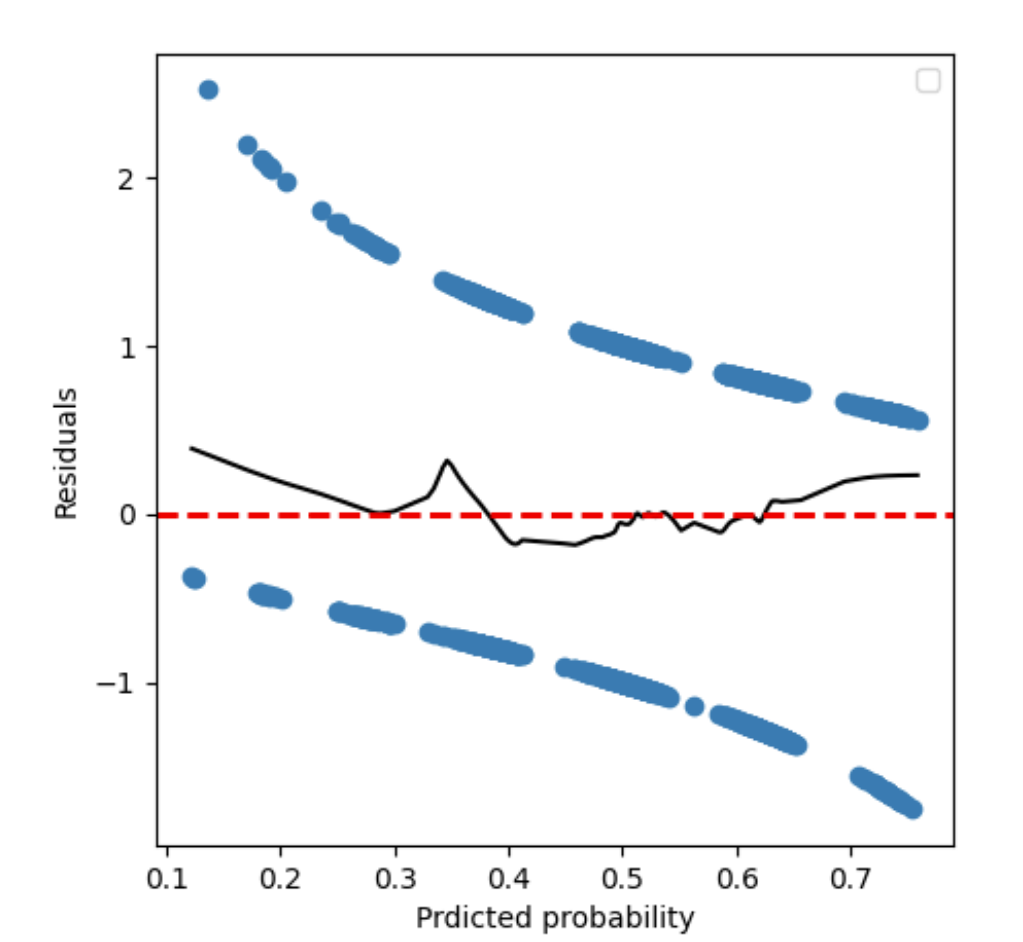
\includegraphics[scale=0.3]{residual_1}
\end{center}
Although the pearson residual vs estimated probability for model 2 shows a curve
close to 0, the pattern in the graph shows that the model did not fit the data well.
Similar to model 1, we attribute this to missing parameters in our model.
\begin{center}
    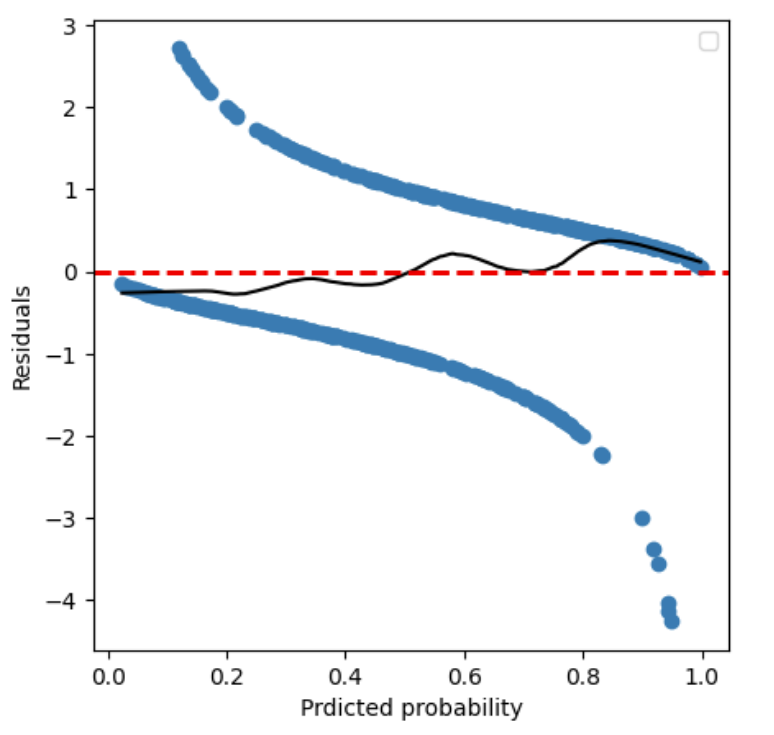
\includegraphics[scale=0.4]{residual_2}
\end{center}

\section{Discussion}
Our analysis indicates that without considering the heroes chosen by players,
the distribution of net worth doesn't seem to affect a team's chance of winning.
However, individual net worth positively influences the probability of winning,
while the number of towers lost by a team has a negative impact. These patterns
hold true across all three game durations we examined.
\\

A significant drawback of our study is not including hero choices as a factor
in our models. Some heroes perform differently against specific opponents, and
hero choices might interact with net worth, affecting our findings. This omission
weakens the reliability of our results.
\\

Both of our models display signs of overdispersion or noticeable patterns in
residual plots. Exploring alternatives to logistic regression or including more
parameters might help improve our results.
\\

Additionally, we couldn't confirm that our models meet the assumption of
linearity. This means our results could change if there are nonlinear factors
affecting the model. It's important to recognize this limitation and consider
potential adjustments in future analyses.

\section{Contribution}
\begin{itemize}
    \item Sathkrith: Hypothesis Testing, Model selection, Model validation, Verification of assumptions, Report.
    \item Madhukara: Data collection, Data pre-processing, Exploratory data analysis, Model selection, Report.
\end{itemize}

\newpage
\section{Appendix}

\appendix

\section{Data visualization to identify key factors}


\label{sec:datavisualization}
\begin{center}
\includegraphics*[scale=0.4]{covar}
\end{center}

\section{AIC test with forward model selection}
\label{sec:aictest}
Akaike Information Criterion is a measure used for statistical model selection,
including logistic regression. It balances the goodness of fit and model complexity,
aiming to identify the model that best explains the data while penalizing for including additional parameters that may not be necessary.
\\

It is calculated as follows:
\[AIC= -2 \times \text{loglikelihood} + 2 \times number\_of\_parameters\]
Lower AIC values indicate a better trade-off between fit and complexity.

\begin{center}
\includegraphics*[scale=0.4]{aic_curve.png}
\end{center}

\section{Interaction tests}
\label{sec:interactiontest}
\begin{center}
\includegraphics*[scale=0.5]{interaction}
\end{center}

\section{Diagnostic tests}
\label{sec:diagnostictest}
\subsection*{ROC Curve}
The Receiver Operating Characteristic (ROC) curve is a graphical representation
used in binary classification to assess and visualize the performance of a
predictive model. It illustrates the trade-off between the true positive rate
(sensitivity) and the false positive rate (1-specificity) across different
threshold values.

The Area Under the ROC Curve (AUC) is a scalar value that quantifies the overall
 performance of the model. A higher AUC indicates better discrimination between
 positive and negative instances.
\begin{center}
    \includegraphics*[scale=0.5]{roc_curve}
    \end{center}

\section{Hypothesis testing for Logistic regression}
We use likelihood ratio test to compare the full and reduced model to determine
if all parameters are zero.
\begin{itemize}
    \item \textbf{Null Hypothesis}: All parameters are zero (not significant)
    \\ \(H_0: \beta_1 = \beta_2 = \dots = \beta_n = 0\)
    \item \textbf{Alternate Hypothesis}: Not all parameters are zero (some are significant)
    \\ \(H_1: \beta_i \neq 0\) for at least one \(i\)
\end{itemize}
\includegraphics*[scale=0.6]{test}
\bibliographystyle{plain}
\bibliography{references}

\end{document}
